\documentclass[zad,zawodnik,lt]{sinol}
  \signature{boi012}
  \id{gat}
  \title{Sklendės}
  \author{Linas Petrauskas}
  \etap{}
  \day{1}
  \date{19--04--2008}
  \RAM{96}                %% Memory limit -- can be skipped in a proposal
  %\Time{}              %% Time limit --  can be skipped in a proposal
  \def\sinolContestLogo{boi08-logo}
  \iomode{stdin}
  \pagestyle{fancy}
  \history{08.03.2008}{[JR] Redakcja}{1.0}
  \history{27.03.2008}{[WT] Uzupelnienie limitow}{1.1}
  \history{06.04.2008}{[MP] Change of guaranteed set of points, minor changes}{1.2}

\begin{document}
  \begin{text}%
Ne vienerius metus dirbęs programuotoju nusprendėte pakeisti darbą ir ėmėte skaityti atsitiktinius darbą siūlančius skelbimus.
Labiausiai Jums užkliuvo pasiūlymas dirbti žuvininkystės ūkyje.
,,Jėga``--- pagalvojote Jūs. Be to, žuvys --- mielos būtybės.
Taigi pasiūlėte savo kandidatūrą, Jus priėmė ir šiandien pirmoji diena naujame darbe.
  
Viršininkas iš karto paskyrė Jums užduotį --- izoliuoti vieną vandens rezervuarą nuo kito.
Išstudijavus duotas schemas, paaiškėjo štai kas.
 
Du vandens rezervuarus jungia keletas kanalų.
Kiekvienas kanalas turi dvi sklendes.
Kanalas atviras tik jei atidarytos abi sklendės, ir uždarytas priešingu atveju.
Kanalo sklendės valdomos jungikliais.
Tas pats jungiklis gali valdyti keletą sklendžių, tačiau kiekvieną sklendę valdo tik vienas jungiklis.
Gali būti, kad abi to paties kanalo sklendes kontroliuoja vienas jungiklis, taip pat --- kad jungiklis nekontroliuoja jokių sklendžių.

    \begin{center}
      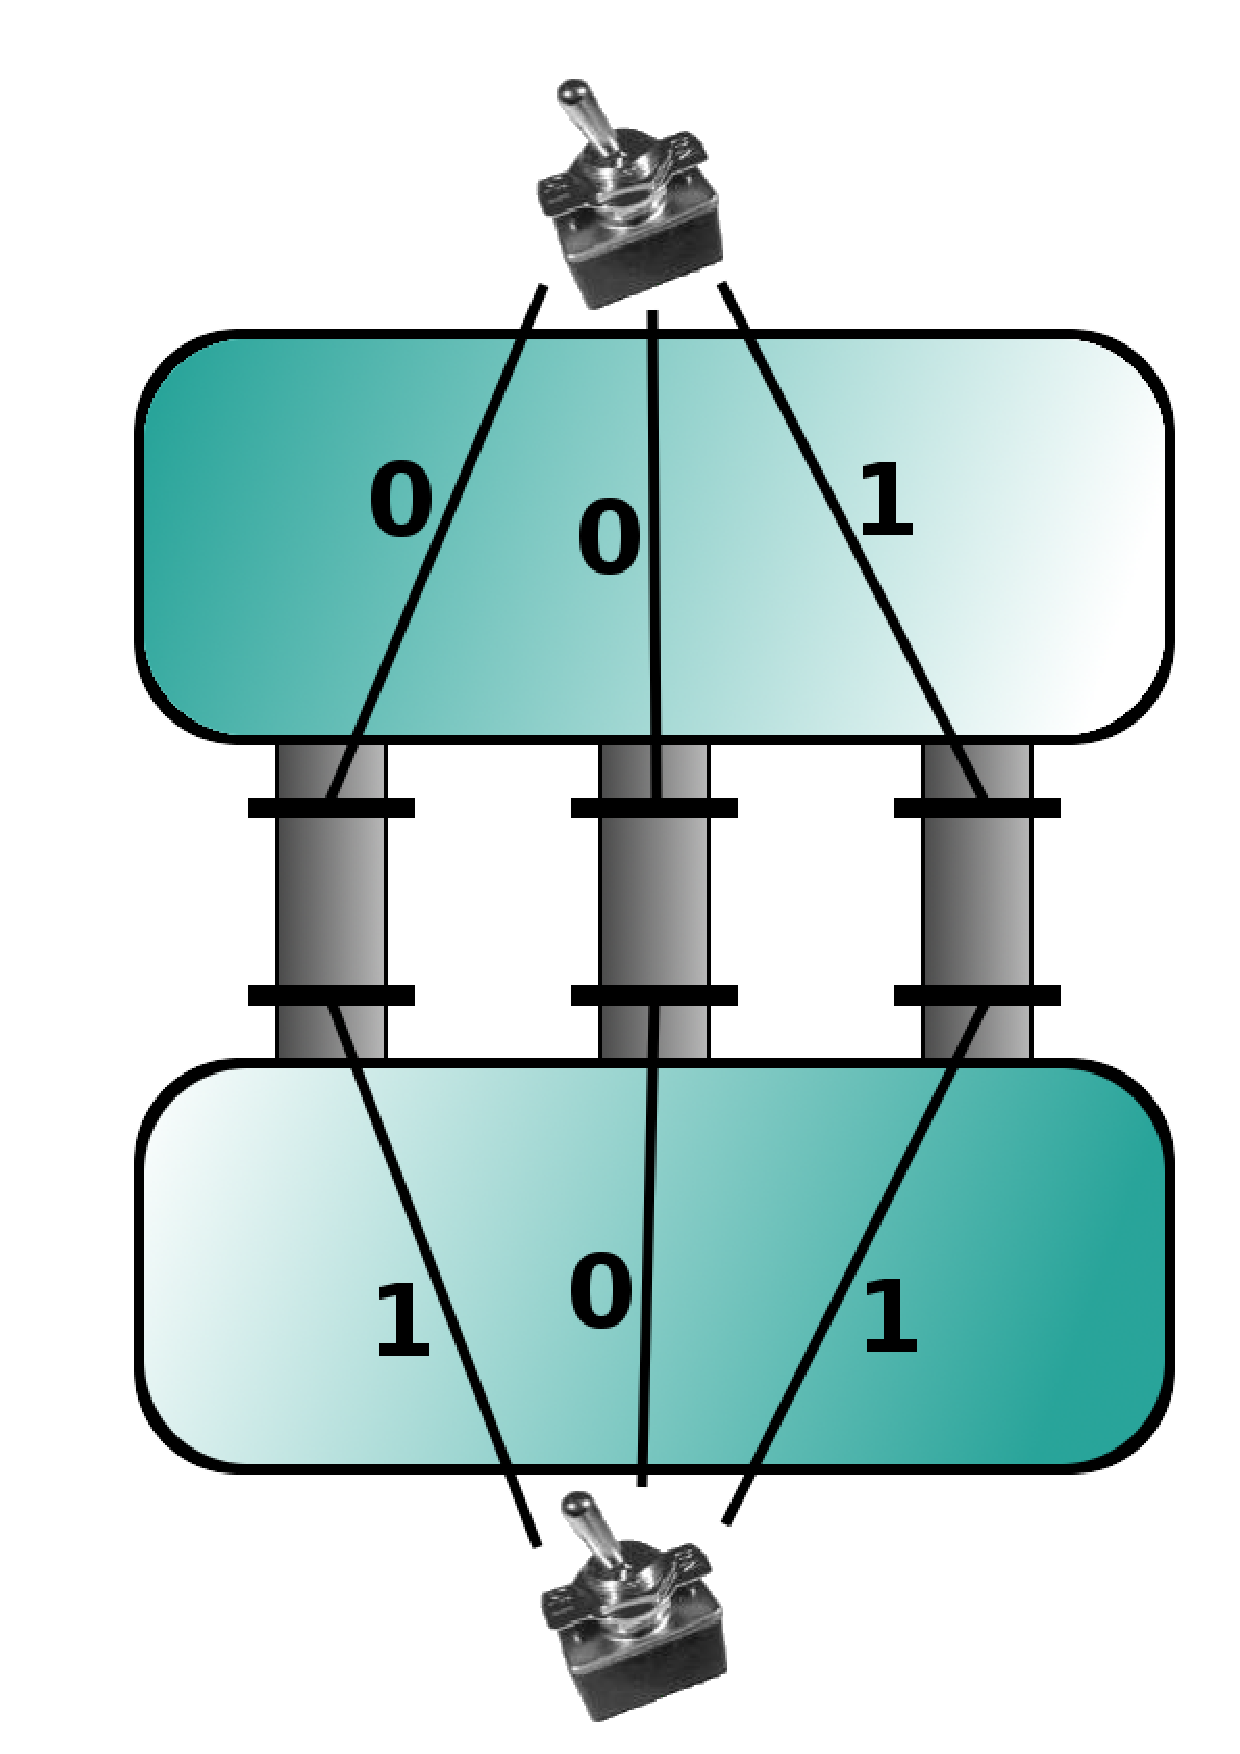
\includegraphics[width=5cm]{gates}\\
      \textit{Pavyzdys su trimis kanalais ir dviem jungikliais.}
    \end{center}
    Kiekvienas jungiklis valdo atitinkamą sklendę vienu iš dviejų būdų:
    \begin{itemize}
      \item
        sklendė atidaryta, kai jungiklis įjungtas, ir uždaryta, kai jis išjungtas,
      \item
        sklendė uždaryta, kai jungiklis įjungtas, ir atidaryta, kai jis išjungtas.
    \end{itemize}

    Šiek tiek pažaidęs su jungikliais staiga suprantate, kad programavimo patirtis čia gali labai praversti.
    Parašykite programą, kuri pagal duotą jungiklių ir sklendžių konfigūraciją nustatytų, ar įmanoma uždaryti visus kanalius, ir jei tai įmanoma, rastų kiekvieno jungiklio padėtį esant uždarytiems visiems kanalams. 
    
    \section{Pradiniai duomenys}
      Pirmoje eilutėje įrašyti du sveikieji skaičiai $n$ $(1 \le n \le 250\,000)$ 
		ir $m$ $(1 \le m \le 500\,000)$ --- tai kanalų ir jungiklių skaičiai, atitinkamai. Jungikliai sunumeruoti nuo 1 iki $m$. Taip pat, testuose, kurių vertė ne mažesnė kaip $30$\% taškų, $n$ neviršys $40$, o $m$ neviršys $20$.		

      Tolesnės $n$ eilučių apibūdina kanalus.
      Kiekvienas kanalas apibūdinamas atskiroje eilutėje keturiais sveikaisiais skaičiais:
      $a$, $s_a$, $b$, $s_b$.
      Skaičiai $a$ ir $b$ nurodo šio kanalo sklendes valdančius jungiklius ($1\le a,b\le m$).
      Skaičiai $s_a$ ir $s_b$ gali būti $0$ arba $1$ --- jie žymi atitinkamos sklendės valdymo režimą:
      $s_i=0$ reiškia, kad sklendė uždaryta tada ir tik tada, kai $i$-asis jungiklis yra išjungtas,
      o $s_i=1$ reiškia, kad sklendė uždaryta tada ir tik tada, kai $i$-asis jungiklis įjungtas.
      
    \section{Rezultatai}
    
      Jei įmanoma uždaryti visus kanalus, į standartinį išvedimo įrenginį turi būti išvesta $m$ eilučių.
      $i$-ojoje eilutėje turi būti įrašytas $0$, jei $i$-asis jungiklis turi būti išjungtas, ir $1$ --- jei jis turi būti įjungtas.
      Jei yra keli galimi sprendiniai, pateikite bet kurį. 

      Jei neįmanoma uždaryti visų kanalų, Jūsų programa turi išvesti vieną eilutę su žodžiu\\ \texttt{IMPOSSIBLE}.

  \makecompactexample

  \twocol{
    ir pradiniams duomenims:
  \iffileexists{\sinolTestIn/\ID0a.in}{%
    \includefile{\sinolTestIn/\ID0a.in}
  }{
    \includefile{\ID0a.in}
  }
  }{
    teisingas rezultatas yra:
    \iffileexists{\sinolTestOut/\ID0a.out}{%
      \includefile{\sinolTestOut/\ID0a.out}
    }{
      \includefile{\ID0a.out}
    }
  }
  \noindent
  Pirmasis pavyzdys atitinka sąlygos paveikslėlį.
  \end{text}
\end{document}
